\documentclass[10pt, a4paper]{article}


%%%%%%%%%%%%%%%%%%%%PACKAGES%%%%%%%%%%%%%%%%%%%%
\usepackage{color}  % add colors to text
\usepackage{microtype} %better letter spacing and etc
\usepackage{titling} %control the typeset of maketitle
%\usepackage[11pt]{moresize}

\usepackage{float} %allows strict placement of a float + override latex replacement -->use H

\usepackage{amsmath}  %pimp your equations
\usepackage{amssymb}  %all those extra math symbols
\usepackage{siunitx} 	% SI units

\usepackage[english]{babel}
%\usepackage[utf8]{inputenc} 
\usepackage[T1]{fontenc}  %font encoding of the input text

\usepackage{graphicx} %import graphs images and whatnot

\usepackage{caption}  %customize figure captions
\usepackage{subcaption}  %create multiple floats within a single environment giving individual captions

\usepackage{tabularx} % x designator for auto expanding width of a table column
\usepackage{tabulary} %better columns for tables: l c r j
\usepackage{booktabs} %get those pretty tables
\usepackage{booktabs} %extra commands for creating stylish tables
\usepackage{arydshln} %drawing dash lines in arrays/tabulars

\usepackage{array}  %more table handling
\usepackage{multirow} %typeset text into multiple rows
\usepackage{wrapfig} %figures with which text can flow around




%%%%%%%%%%%%%%%%%%%%PAGE FORMATTING AND WHAT NOT%%%%%%%%%%%%%%%%%%%%
\usepackage[twocolumn,hmargin=2cm,vmargin=2.5cm]{geometry}% rm if title --> full width span when 2column format


%%%%%%%%%%%%%%%%%%%%MACRO DOODLES%%%%%%%%%%%%%%%%%%%%


%%%%%%%%%%%%%%%%%%%%ABREVIATIONS AND DEFINITIONS%%%%%%%%%%%%%%%%%%%%

\def \tss {\textsuperscript}



%%%%%%%%%%%%%%%%%%%%PATHS%%%%%%%%%%%%%%%%%%%%

\graphicspath{{../src/}{.}{src/}}	



%%%%%%%%%%%%%%%%%%%%TITLE%%%%%%%%%%%%%%%%%%%%


%\author{Bian Theophile, Mathias Dankl, Mercan Samuele}
\pretitle{\begin{center}
	\vspace*{-3cm}
	
\includegraphics[scale = 0.2]{epfl_nonofficial_logo.png}\\[1cm]}
%\title{\large{\textbf{Deep Learning -- EE559 \\ Mini Neural Network Framework}}}
\posttitle{\end{center}}


%%%%%%%%%%%%%%%%%%%%DOCUMENT%%%%%%%%%%%%%%%%%%%%
\begin{document}
\title{\large{\textbf{Deep Learning -- EE559 \\ Mini Neural Network Framework}}}
\date{\normalsize{\today}}
%date of report: 17/05/2019
\author{\normalsize{Th\' eophile 	\sc{Bian}} \and \normalsize{Mathias \sc{Dankl}} \and \normalsize{Samuele \sc{Mercan}}}
\maketitle
%MODIFY FIG1
\section{Introduction:} 
The goal of this project is to design and implement a framework which substitutes some of the PyTorch framework's functionalities. This mini "deep-learning framework" uses some of the more basic PyTorch components such as tensor operations, but does without the forward, backward, autograd, neural modules and other functions. 
The main task the framework should be able to achieve is to create a specific network, train it, and compute the training and testing errors.
In particular, the specific network architecture to be implemented consists of a network with two input units, two output units, three hidden layers of 25 units, and should be trained with mean-square loss (MSE) and stochastic gradient descent (SGD) optimization.
The dataset is generated within the code. The data consists of a train and test set of 1000 points, sampled uniformly within $[0,1]$x$[0,1]$. The label is set to 1 if the point is within a disk of radius $\sqrt{\frac{1}{2\pi}}$, and 0 if not. Therefore the specific task at hand is to create a classifier for non-linearly separable binary data, even though the framework should be capable of dealing with other types of datasets and tasks.
	
\section{Architecture:}The main idea behind the framework detailed here is that even though the code implemented does not fully supplement the PyTorch functionalities, the overall architecture is flexible and modular enough to allow expansion and add-ons to do that. In this case, because of 	the specific network requirements -- an MLP-type model, with fully connected layers -- a Convolutional Layer Module or Recursive Layer Module was not implemented. The framework is structured so that new, specific layer types can be implemented and used to create a network. Loss functions and optimizers can also be added on.

The framework can be split into two major parts: a network-building part, and a complementary part (cf. Fig.~\ref{fig:arch_org}). 
\paragraph{Network Creation}
On one side, network modules are defined as classes, each class containing its own methods especially an initiation method called upon instance creation. There are two types of network classes: Module and Sequential. A Sequential instance is defined as an ordered list, or sequence, of Module instances, defining the global network architecture. There is also an Optimizer class, defining the weights optimization method. 
\begin{figure}
	\begin{centering}
		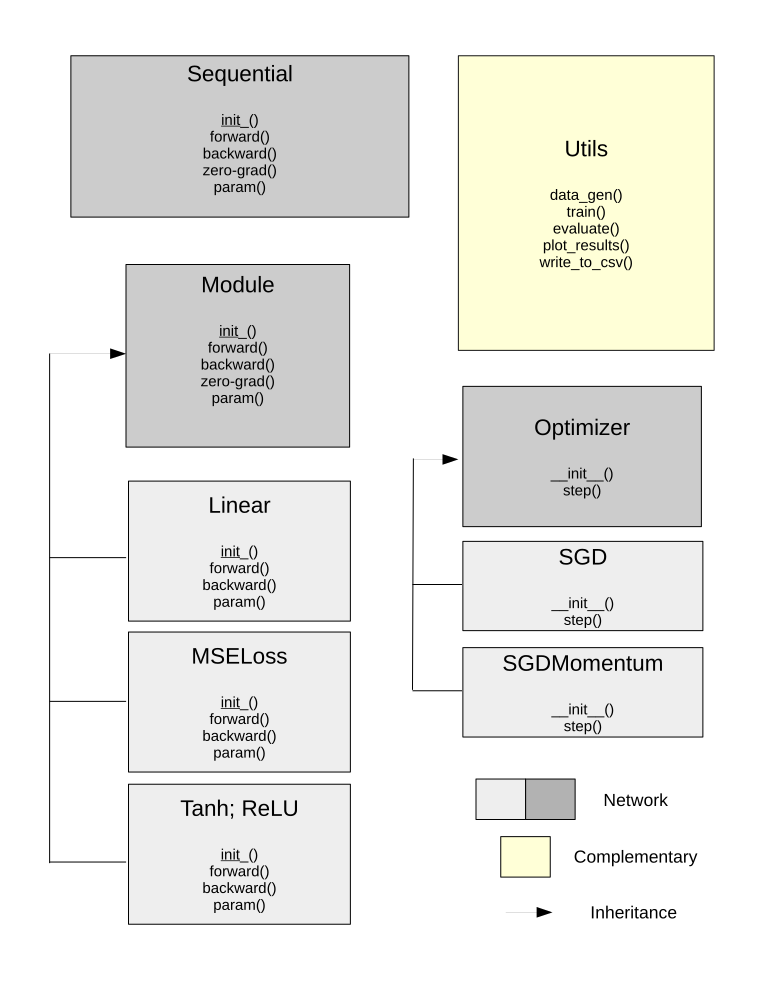
\includegraphics[scale=0.4]{architecture_org.png}
		\caption{Framework Architecture Organigram}
		\label{fig:arch_org}
	\end{centering}
\end{figure}

The Module class is the base building block of our network, and contains the forward, backward, and parameter functions. In order to maintain a high degree of modularity, a parent class was defined with loose attributes and methods. The children classes can be divided into several subclass types: Layers, Activation Functions, and Losses. The children classes override the parent class methods and attributes.
\begin{itemize}
\item Layers: specifically a linear layer module named Linear, which defines what a standard MLP is. This layer module can be tailored to one's needs, with variable input and output size. It is a fully connected layer but weight initialization can be set, in order to be able to implement weight sharing. 
It contains several methods: init() which instantiates the layer; forward() which computes the output of a layer; backward() which computes the backward propagation of errors through a layer; param() which returns the layer's weights, biases and their respective gradients; zero\_grad() which iterates on its parameter gradients and sets them to zero; and optimize() which updates the weights according to the given criterion.
The gradient re-setting function is implemented in the same way as the training one, meaning that the overall model's zero\_grad() function iterates on its components and calls their own zero\_grad() methods (thus each layer's gradient is reset).

\item Activation Functions: notably Tanh and ReLU. These activation functions were created as part of the Module class to be able to run the whole network's forward and backward passes by iterating on each of its components.

\item Loss Functions: MSE loss in particular. Losses were defined as Module subclasses for the same reasons as activation functions.
\end{itemize}
The idea behind having these different components inherit the same class is that this way they can share the same main forward, backward and methods needed to run/train the model properly. More specifically, the forward method can be called similarly for a fully connected layer, an activation function or a loss function.
For the backward pass, this also allows us to circumvent the lack of a method similar to autograd. There is no need to implement a method allowing derivation of any component, in this case derivatives are explicitly set within each children class backward pass method.

The Sequential class is a class that allows the piecing of several network blocks, thereby enabling the creation of a custom network. The class initiation method creates the ordered sequence of network components, as one would read it from initial input to final output. It takes a set of parameters in order to define the sequence: first a fully connected layer, than an activation layer, and so on.

The loss function is not used in the model creation. This was designed such as to enable the comparison of different loss functions on one model externally. However, since the method needs to make use of the backward functionality of the network, it was designed as being a child of the Module class.

An optimizer class was created, with some children classes such as SGD and SGD with momentum; more could be added (Adam optimizer, etc…). A parent class was created because all optimizers will be used in the same way: initialization with a set of parameters/weights, and update with a specific rule. The optimizer fetches parameters from the model using the param() method.


\subparagraph{Complementary Functions:}
On the other side, there are a number of supporting functionalities. To be able to train and test the model, another set of functions were created. These can be found in the Utils file. This file contains the model training method, a flexible functionality that can be called on with any model and any loss criterion. The testing method is implemented similarly. These two methods aim to replace the training method implemented in the PyTorch module, namely model.train() and model.eval(). A similar structure was implemented, with the training method computing an output by executing the forward pass of each element within the model in the order they are given -- while logging the intermediary results -- then computing the loss according to the specified criterion (MSE in this case). The loss gradients (w.r.t. the weights) are reset, then the backward pass is computed through each model element in the reverse order. The optimizer is then used to update the weights accordingly. Losses are logged and the final parameters are returned. Looping is implemented to be able to train the model on different epochs. A batching system is also put in place. This training method is specific to a certain type of loss (trying to minimize loss function, not maximize likelihood). These methods are implemented specifically for a 2D dataset and a classification task.

The testing method is similar to the training one in its architecture, and of course only consists of a forward pass and no updating of weights is done, similar to the model.eval() function in PyTorch. The number of errors is logged. 
The Utils file contains the method used for data generation. This complementary file also contains data plotting functions both for the input dataset and the output dataset, which are both specific to the dataset generated in the same file.
The network is instantiated through a file named test.py, which first defines the network characteristics (architecture, loss function used, optimizer, input dataset -- both for training and testing, number of epochs for training, data-batching size) then trains the model, and tests its accuracy in classification. 


\section{Performance:}A first round of testing was performed, based on model creation parameters. Different  learning rates, epochs, standard deviations (for weight and bias layer initialization), number of nodes within layers and number of layers, as well as activation functions were used to run iterations of the network. This round of testing aimed to confirm that the evolution of parameters was consistent with what was theoretically expected; both in overall prediction accuracy, losses evolution, and physical training and testing time. 
%<<NEED TO ACTUALLY RUN THIS….  AND INCLUDE RESULTS – 1 graph/table is sufficient>>
It is important to note that this series of tests is limited and is in no way exhaustive but only aims to provide a sense of the framework's ability at performing a single definite task.
Since the performance was the main aspecct of the framework development, model hyperparameters tuning was not explored.
\paragraph{Model Comparison:}
\begin{figure}[H]
	\begin{centering}
		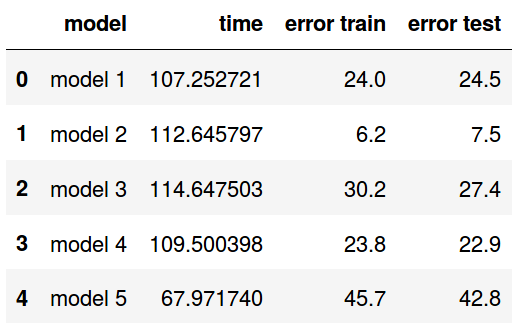
\includegraphics[scale=0.3]{model_subs.png}
		\caption{Model Comparison}
		\label{fig:model_subs}
	\end{centering}
\end{figure}
\footnotesize{Parameters for all models: eta = 0.1; epochs = 100; n\_ train = 1000; n\_ test = 1000\\
Model 1: 3 Fully Connected Layers, 25 nodes per layer, ReLU activation \\
Model 2: 3 Fully Connected Layers, 25 nodes per layer, Tanh activation \\
Model 3: 3 Fully Connected Layers, 50 nodes per layer, Tanh activation \\
Model 4: 3 Fully Connected Layers, 10 nodes per layer, Tanh activation \\
Model 5: 1 Fully Connected Layer, 20 nodes per layer, Tanh activation \\}

\section{Submission} The submission file is slightly different from what is detailed here. The architecture is identical, and the code is more raw, with for example no plotting and no iteration over parameters. 


\section{Discussion}The framework implemented remain simple enough that it can be expanded only through the creation of new classes and child classes. For instance, the implementation of a dropout feature could be done within the Linear class, by adding an attribute specifying the dropout rate. In the model's forward and backward pass methods, based on the attribute value, the dropout feature could be run/not. Similarly, for a Convolutional Layer, a whole new child class could be implemented with its own features. 
This advantage is also an inconvenience since it creates some redundancy in the code. 
The framework itself is limited because of the lack of different modalities implemented. It is also penalized by its explicitness and its lack of modularity.
The most obvious examples are the training and testing methods which are implemented with respect to the classification task at hand, and with respect to the loss considered. These methods can be improved and modularized. 




\end{document}

